% Registrazione alla WebApp
Registrarsi su Sweeat è un’operazione semplice, gratuita e disponibile a chiunque, la quale permette all’utente di creare un account all’interno della piattaforma dove realizzare una lista dei preferiti e suggerire profili Instagram.

È possibile accedere al modulo di registrazione tramite il seguente link:

\begin{center}
\textsl{ \href{https://dev.d1ay0almkohcfw.amplifyapp.com/registrazione}{\textbf{https://dev.d1ay0almkohcfw.amplifyapp.com/registrazione} }}
\end{center}

Per registrarsi su Sweeat è necessario cliccare sul bottone “\textbf{Registrati}” nella barra di navigazione (in alto a destra nella versione Desktop e nel bottone presente all'interno del menù a tendina nella versione mobile).

\begin{figure}[H]
\centering

\includegraphics[scale=0.15]{./images/Registrazione/RegDesktop.png} 
\caption{Bottone di registrazione versione desktop}
\end{figure}

\begin{figure}[H]
\centering
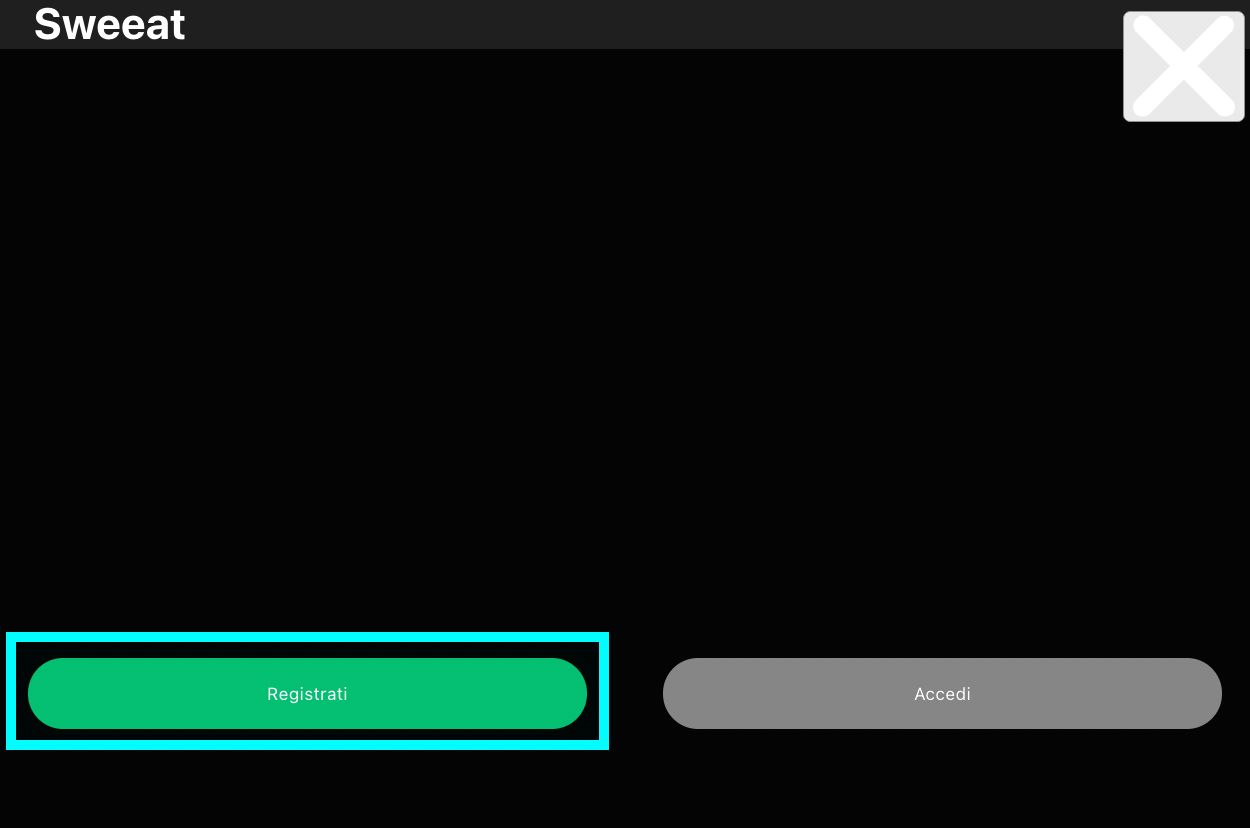
\includegraphics[scale=0.2]{./images/Registrazione/RegMobile.png} 
\caption{Bottone di registrazione versione mobile}
\end{figure}

Una volta cliccato sul bottone, l’utente verrà reindirizzato in una nuova pagina contenente un modulo, nel quale dovrà inserire i dati per la registrazione.

\begin{figure}[H]
\centering
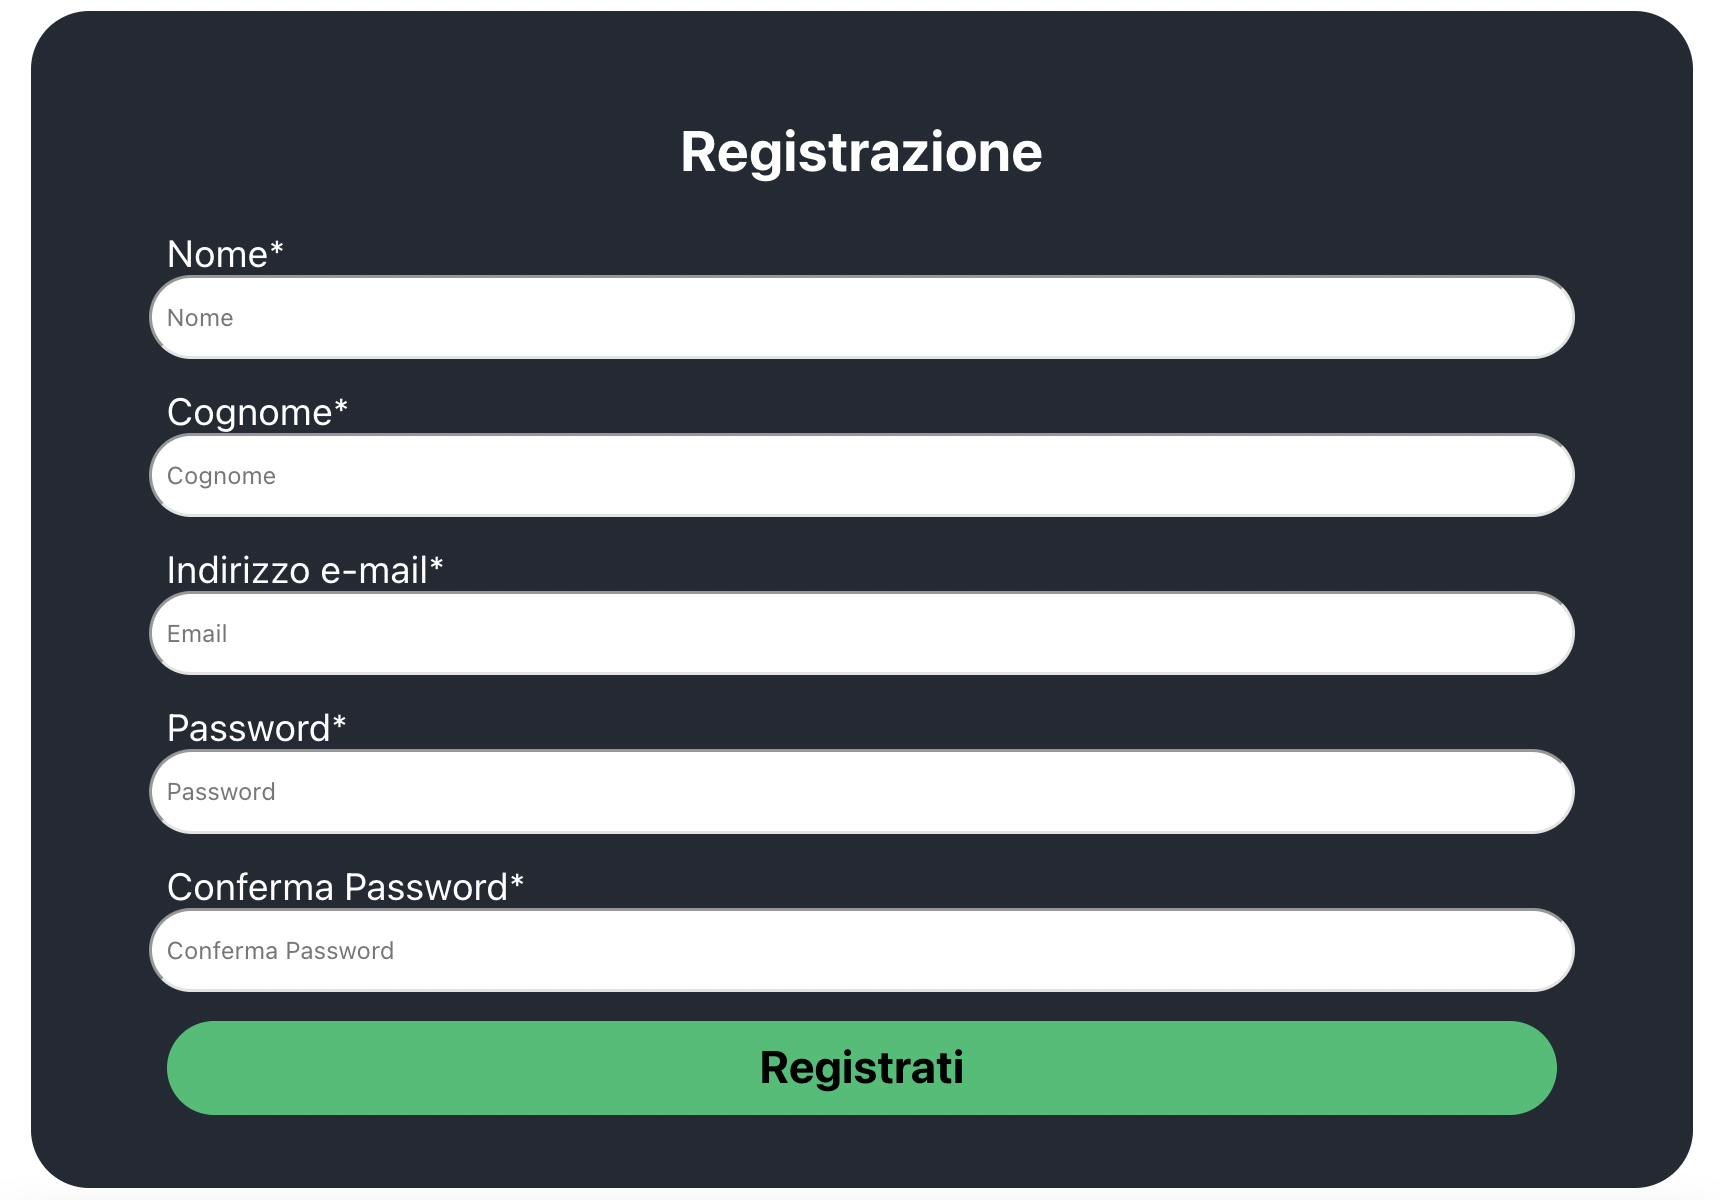
\includegraphics[scale=0.3]{./images/Registrazione/FormRegistrazione.png} 
\caption{Modulo di registrazione a Sweeat}
\end{figure}

I dati(*) da inserire in fase di registrazione sono:

\begin{itemize}
\item \textbf{Nome},
\item \textbf{Cognome},
\item \textbf{Indirizzo e-mail}, 
\item \textbf{Password}, (che dovrà essere lunga almeno 8 caratteri e contenere almeno una lettera maiuscola, una minuscola, un numero ed un simbolo tra i seguenti: @ \$ ! \% * ? \&). 
\end{itemize}

(*) tutti i dati richiesti sono obbligatori. \\

L’indirizzo e-mail e la password serviranno per accedere all'account personale nella piattaforma.

Dopo aver inserito tutti i dati richiesti, per effettuare la registrazione sarà necessario cliccare sul bottone “\textbf{Registrati}”.

Una volta fatto ciò, comparirà il seguente messaggio di benvenuto: 

\begin{figure}[H]
\centering

\includegraphics[scale=0.5]{./images/Registrazione/Welcome.png} 
\caption{Messaggio di Benvenuto su Sweeat}
\end{figure}

e sarà necessario confermare la propria identità cliccando sul link che verrà inviato all’indirizzo e-mail inserito in fase di registrazione.

\begin{figure}[H]
\centering

\includegraphics[scale=0.5]{./images/Registrazione/emailReg.png} 
\caption{E-mail di conferma dell'identità}
\end{figure}

Una volta confermato l’account, comparirà il seguente messaggio di conferma:

\begin{figure}[H]
\centering
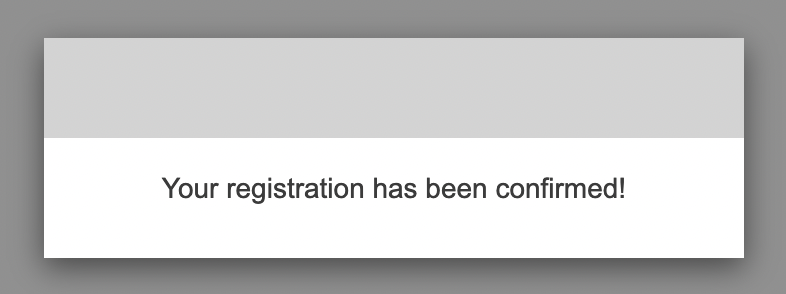
\includegraphics[scale=0.5]{./images/Registrazione/Conferma.png} 
\caption{Conferma di avvenuta registrazione su Sweeat}
\end{figure}

e sarà possibile accedere alla propria \textbf{Area Personale}.

\subsection{Inserimento Dati Errati}

Nel caso in cui l'utente voglia procedere con la registrazione lasciando uno o più campi vuoti, la registrazione non andrà a buon fine ed il sistema mostrerà i seguenti errori:

\begin{figure}[H]
\centering
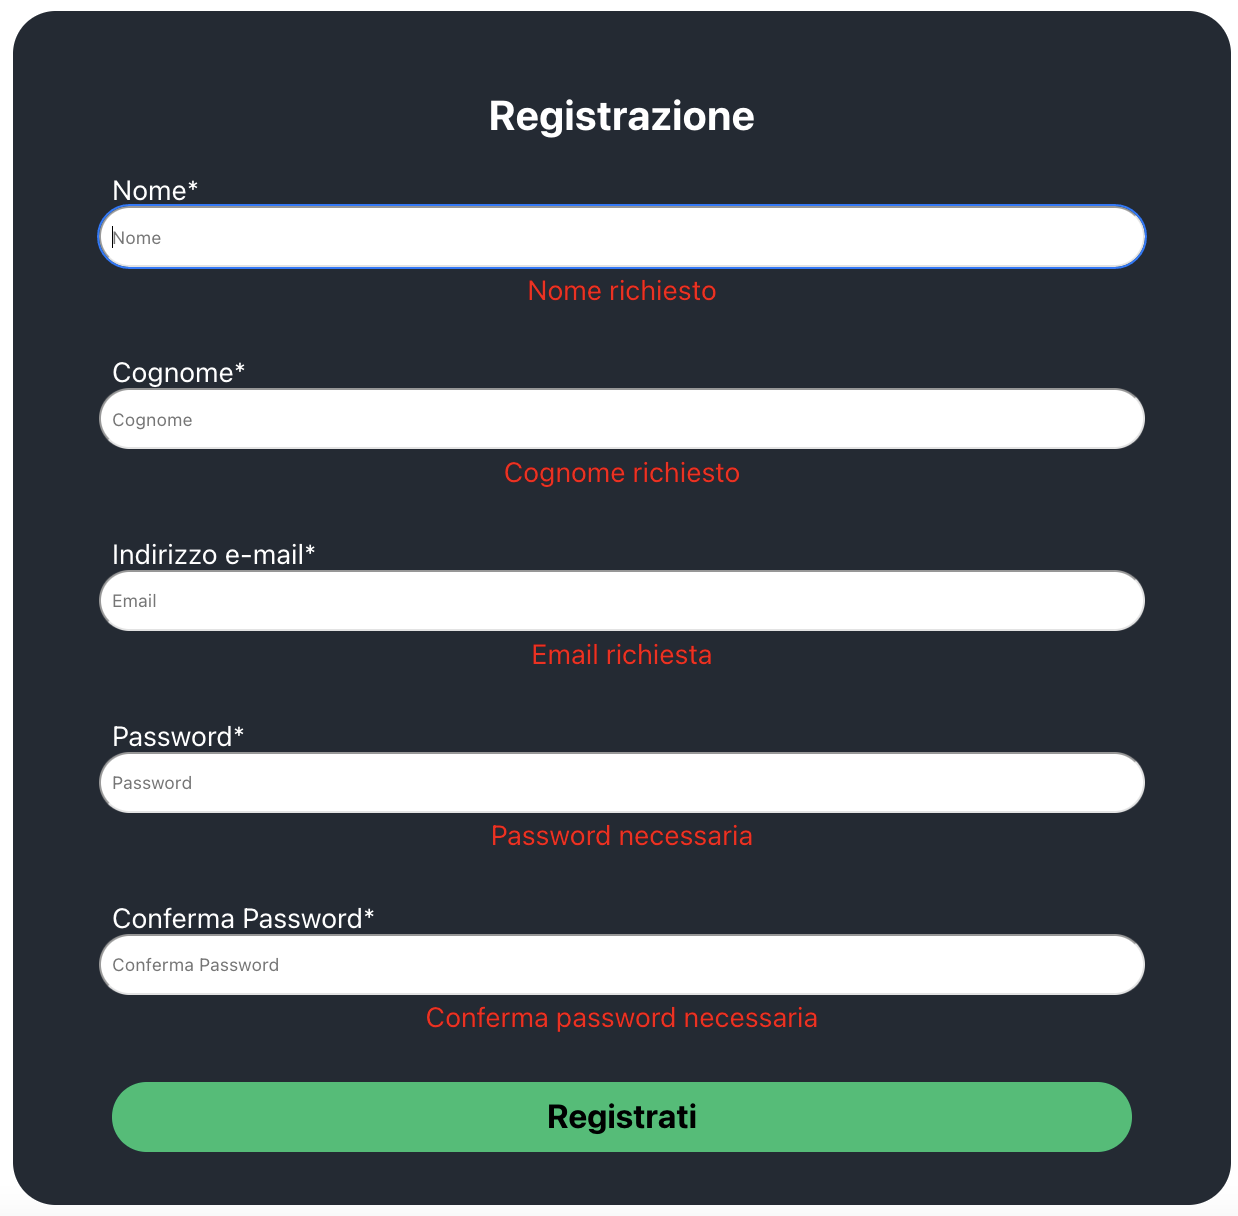
\includegraphics[scale=0.4]{./images/Registrazione/DatiErrati.png} 
\caption{Errori nell'inserimento dei dati in fase di registrazione}
\end{figure}

Affinché la registrazione vada a buon fine, è necessario compilare correttamente tutti i campi. 
